\documentclass[aspectratio=169]{beamer}

% Forest-themed palette matching the PPTX
\usetheme{Madrid}
\usecolortheme{whale}

\definecolor{fvsgreen}{RGB}{44,95,45}
\definecolor{fvsmoss}{RGB}{151,188,98}
\definecolor{fvsdark}{RGB}{30,58,30}
\definecolor{fvscream}{RGB}{245,245,240}
\definecolor{fvsmuted}{RGB}{74,85,104}

\setbeamercolor{structure}{fg=fvsgreen}
\setbeamercolor{frametitle}{bg=fvsdark,fg=white}
\setbeamercolor{title}{bg=fvsdark,fg=white}
\setbeamercolor{block title}{bg=fvsgreen,fg=white}
\setbeamercolor{block body}{bg=fvscream}
\setbeamercolor{item}{fg=fvsgreen}
\setbeamercolor{background canvas}{bg=fvscream}

\setbeamerfont{title}{series=\bfseries,size=\LARGE,family=\rmfamily}
\setbeamerfont{frametitle}{series=\bfseries,family=\rmfamily}

\setbeamertemplate{navigation symbols}{}

\setbeamertemplate{footline}{
  \leavevmode%
  \hbox{%
    \begin{beamercolorbox}[wd=.4\paperwidth,ht=2.25ex,dp=1ex,left]{author in head/foot}%
      \hspace*{2ex}\usebeamerfont{author in head/foot}\insertshortauthor
    \end{beamercolorbox}%
    \begin{beamercolorbox}[wd=.3\paperwidth,ht=2.25ex,dp=1ex,center]{title in head/foot}%
      \usebeamerfont{title in head/foot}\color{fvsgreen}\insertshorttitle
    \end{beamercolorbox}%
    \begin{beamercolorbox}[wd=.3\paperwidth,ht=2.25ex,dp=1ex,right]{date in head/foot}%
      \usebeamerfont{date in head/foot}\insertframenumber{} / \inserttotalframenumber\hspace*{2ex}
    \end{beamercolorbox}}%
  \vskip0pt%
}

\usepackage{graphicx}
\usepackage{booktabs}
\usepackage{tikz}
\usetikzlibrary{arrows.meta,positioning,shapes.geometric}

% Figure path
\graphicspath{{../output/comparisons/manuscript_figures/}}

\title{FVS--Modern}
\subtitle{Bayesian Calibration of the Forest Vegetation Simulator Across CONUS}
\author{Greg Johnson \and David Marshall \and Aaron Weiskittel}
\date{GMUG Meeting \textbar{} April 2026}

\begin{document}

% ============================================================================
% SLIDE 1: Title
% ============================================================================
{
\setbeamercolor{background canvas}{bg=fvsdark}
\begin{frame}[plain]
\vspace{1.5cm}
{\usebeamerfont{title}\usebeamercolor[fg]{title}\Huge\bfseries FVS--Modern}\\[0.6cm]
{\large\color{fvsmoss} Bayesian Calibration of the Forest Vegetation Simulator Across CONUS}\\[1.5cm]
{\color{fvscream} Greg Johnson~~|~~David Marshall~~|~~Aaron Weiskittel}\\[0.3cm]
{\color{fvsmoss!60!fvsdark}\small GMUG Meeting~~|~~April 2026}
\vfill
\begin{tikzpicture}[remember picture,overlay]
  \fill[fvsmoss] (current page.south west) rectangle ([yshift=0.6cm]current page.south east);
\end{tikzpicture}
\end{frame}
}

% ============================================================================
% SLIDE 2: Calibration Workflow
% ============================================================================
\begin{frame}
\frametitle{Calibration Workflow}

\begin{center}
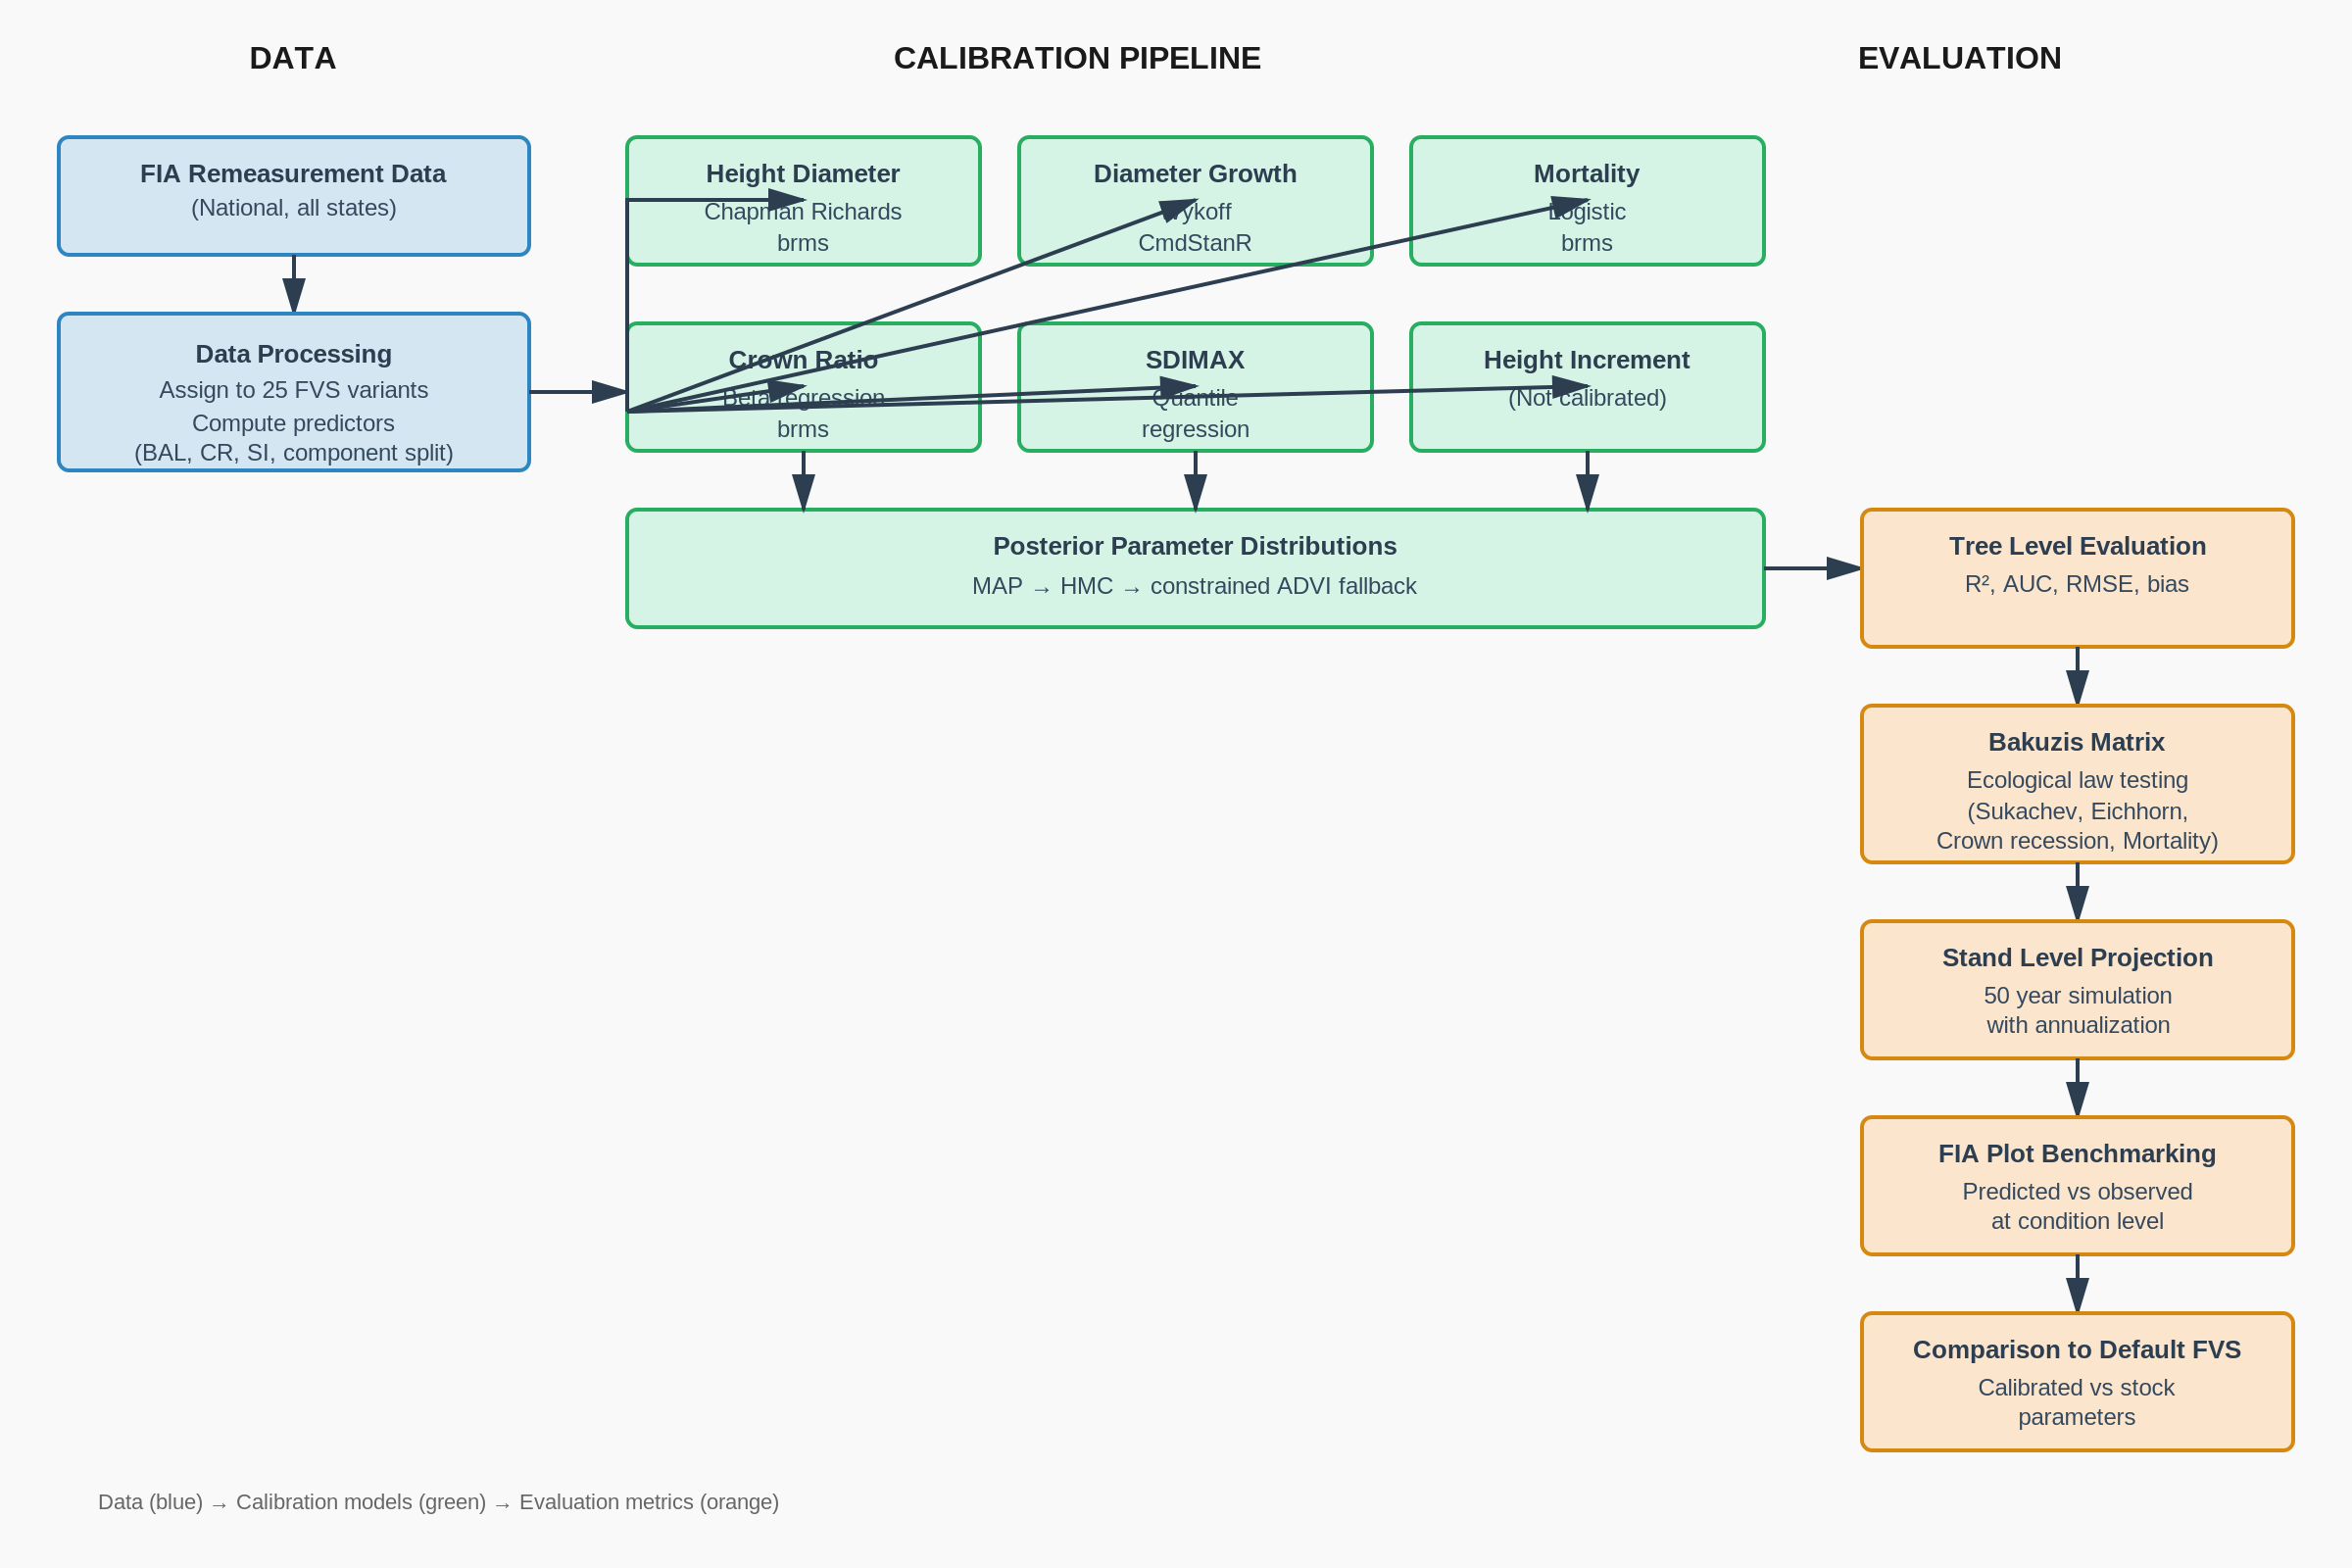
\includegraphics[width=0.92\textwidth]{fig_conceptual_diagram.png}
\end{center}

\vfill
{\scriptsize\color{fvsmuted} 16.2M FIA trees~~|~~435K condition pairs~~|~~25 FVS variants~~|~~Bayesian posteriors via Stan/ADVI}
\end{frame}

% ============================================================================
% SLIDE 3: Performance Heatmap
% ============================================================================
\begin{frame}
\frametitle{Model Performance by Variant and Component}

\begin{columns}[T]
\begin{column}{0.55\textwidth}

\includegraphics[width=\textwidth]{fig_calibration_heatmap.png}
\end{column}

\begin{column}{0.42\textwidth}
\textbf{\color{fvsdark}25 variants calibrated}\\
H--D strongest component ($R^2 = 0.75$--$0.90$)

\vspace{0.4cm}
\textbf{\color{fvsdark}Mortality AUC 0.66--0.93}\\
Large--tree U--shaped mortality now captured in most variants

\vspace{0.4cm}
\textbf{\color{fvsdark}Crown ratio weakest ($R^2 = 0.14$--$0.38$)}\\
Observed CR used at initialization; only change modeled

\vspace{0.4cm}
\textbf{\color{fvsdark}DG $R^2 = 0.30$--$0.69$}\\
Shared 13--covariate Wykoff $\ln(\text{DDS})$ equation with species random effects
\end{column}
\end{columns}
\end{frame}

% ============================================================================
% SLIDE 4: Stand-Level Validation
% ============================================================================
\begin{frame}
\frametitle{Stand--Level Validation: FIA Benchmark}

\begin{center}
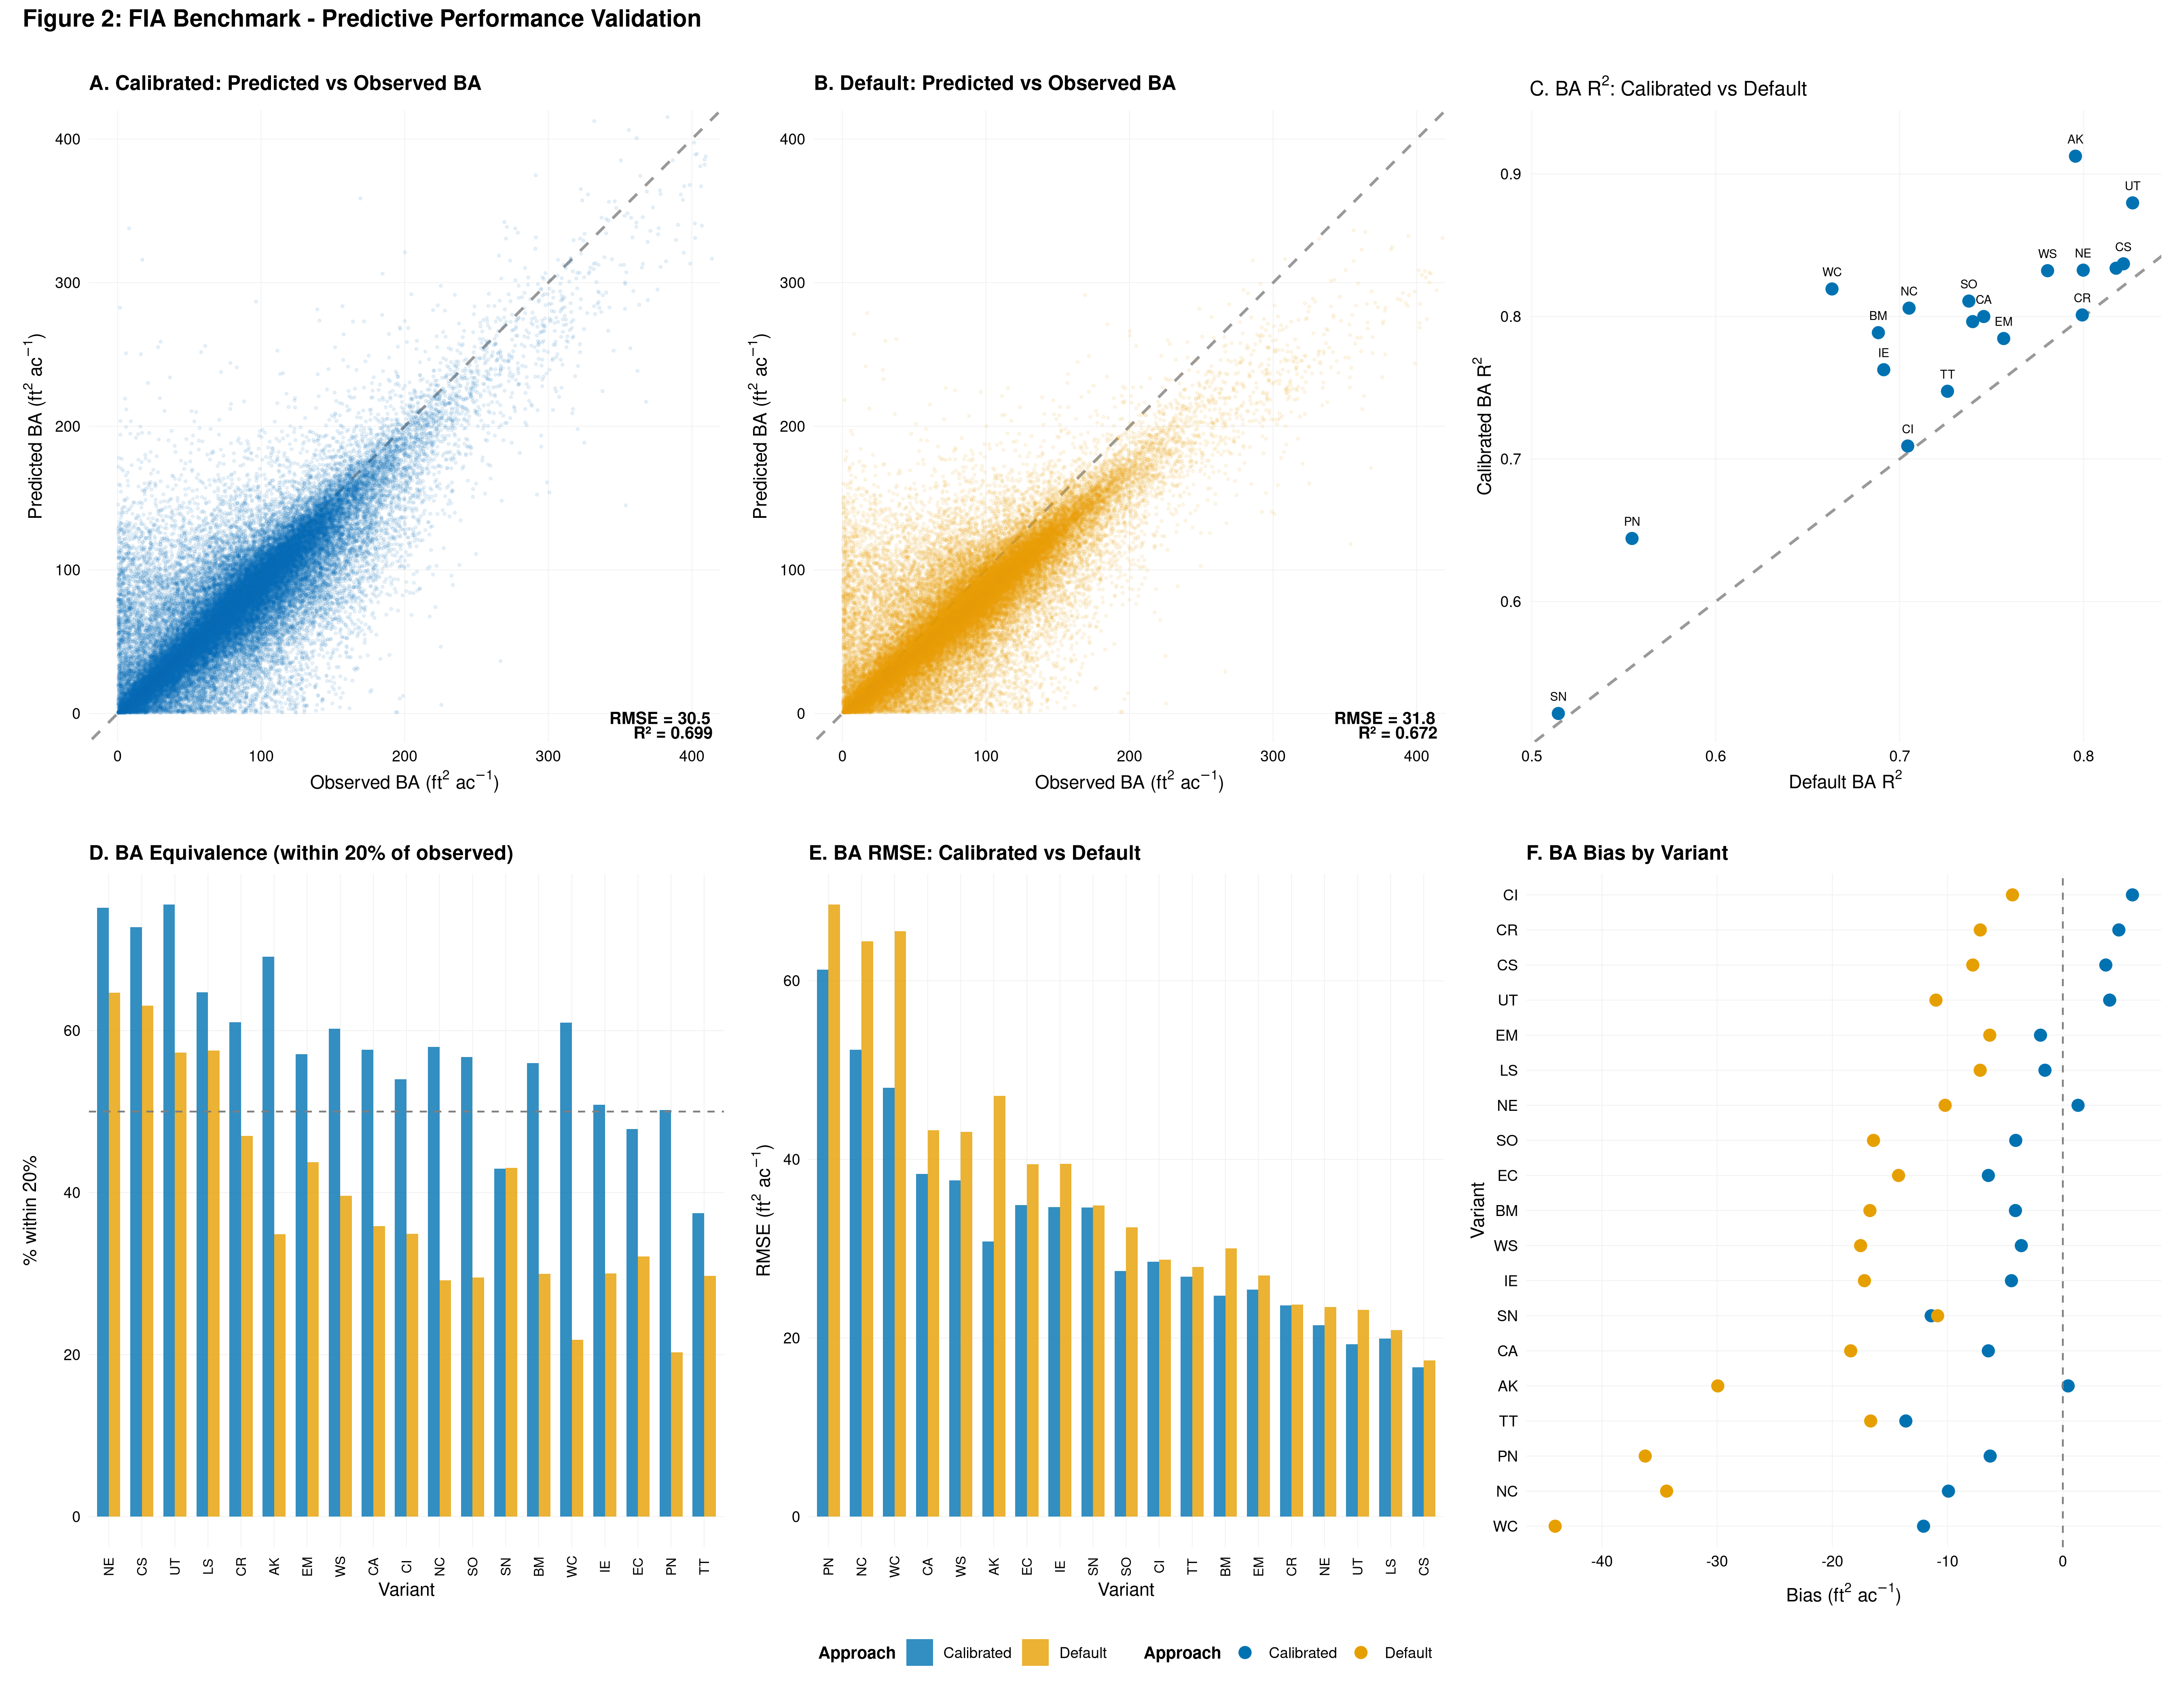
\includegraphics[width=0.95\textwidth]{fig2_fia_benchmark.png}
\end{center}

\vspace{-0.1cm}
{\scriptsize\color{fvsmuted} Predicted vs.\ observed BA for 435K FIA condition pairs. Calibrated (blue) outperforms default (gold) in RMSE, $R^2$, and equivalence across all 19 tested variants.}
\end{frame}

% ============================================================================
% SLIDE 5: RMSE with Uncertainty
% ============================================================================
\begin{frame}
\frametitle{BA RMSE with Bootstrap Confidence Intervals}

\begin{center}
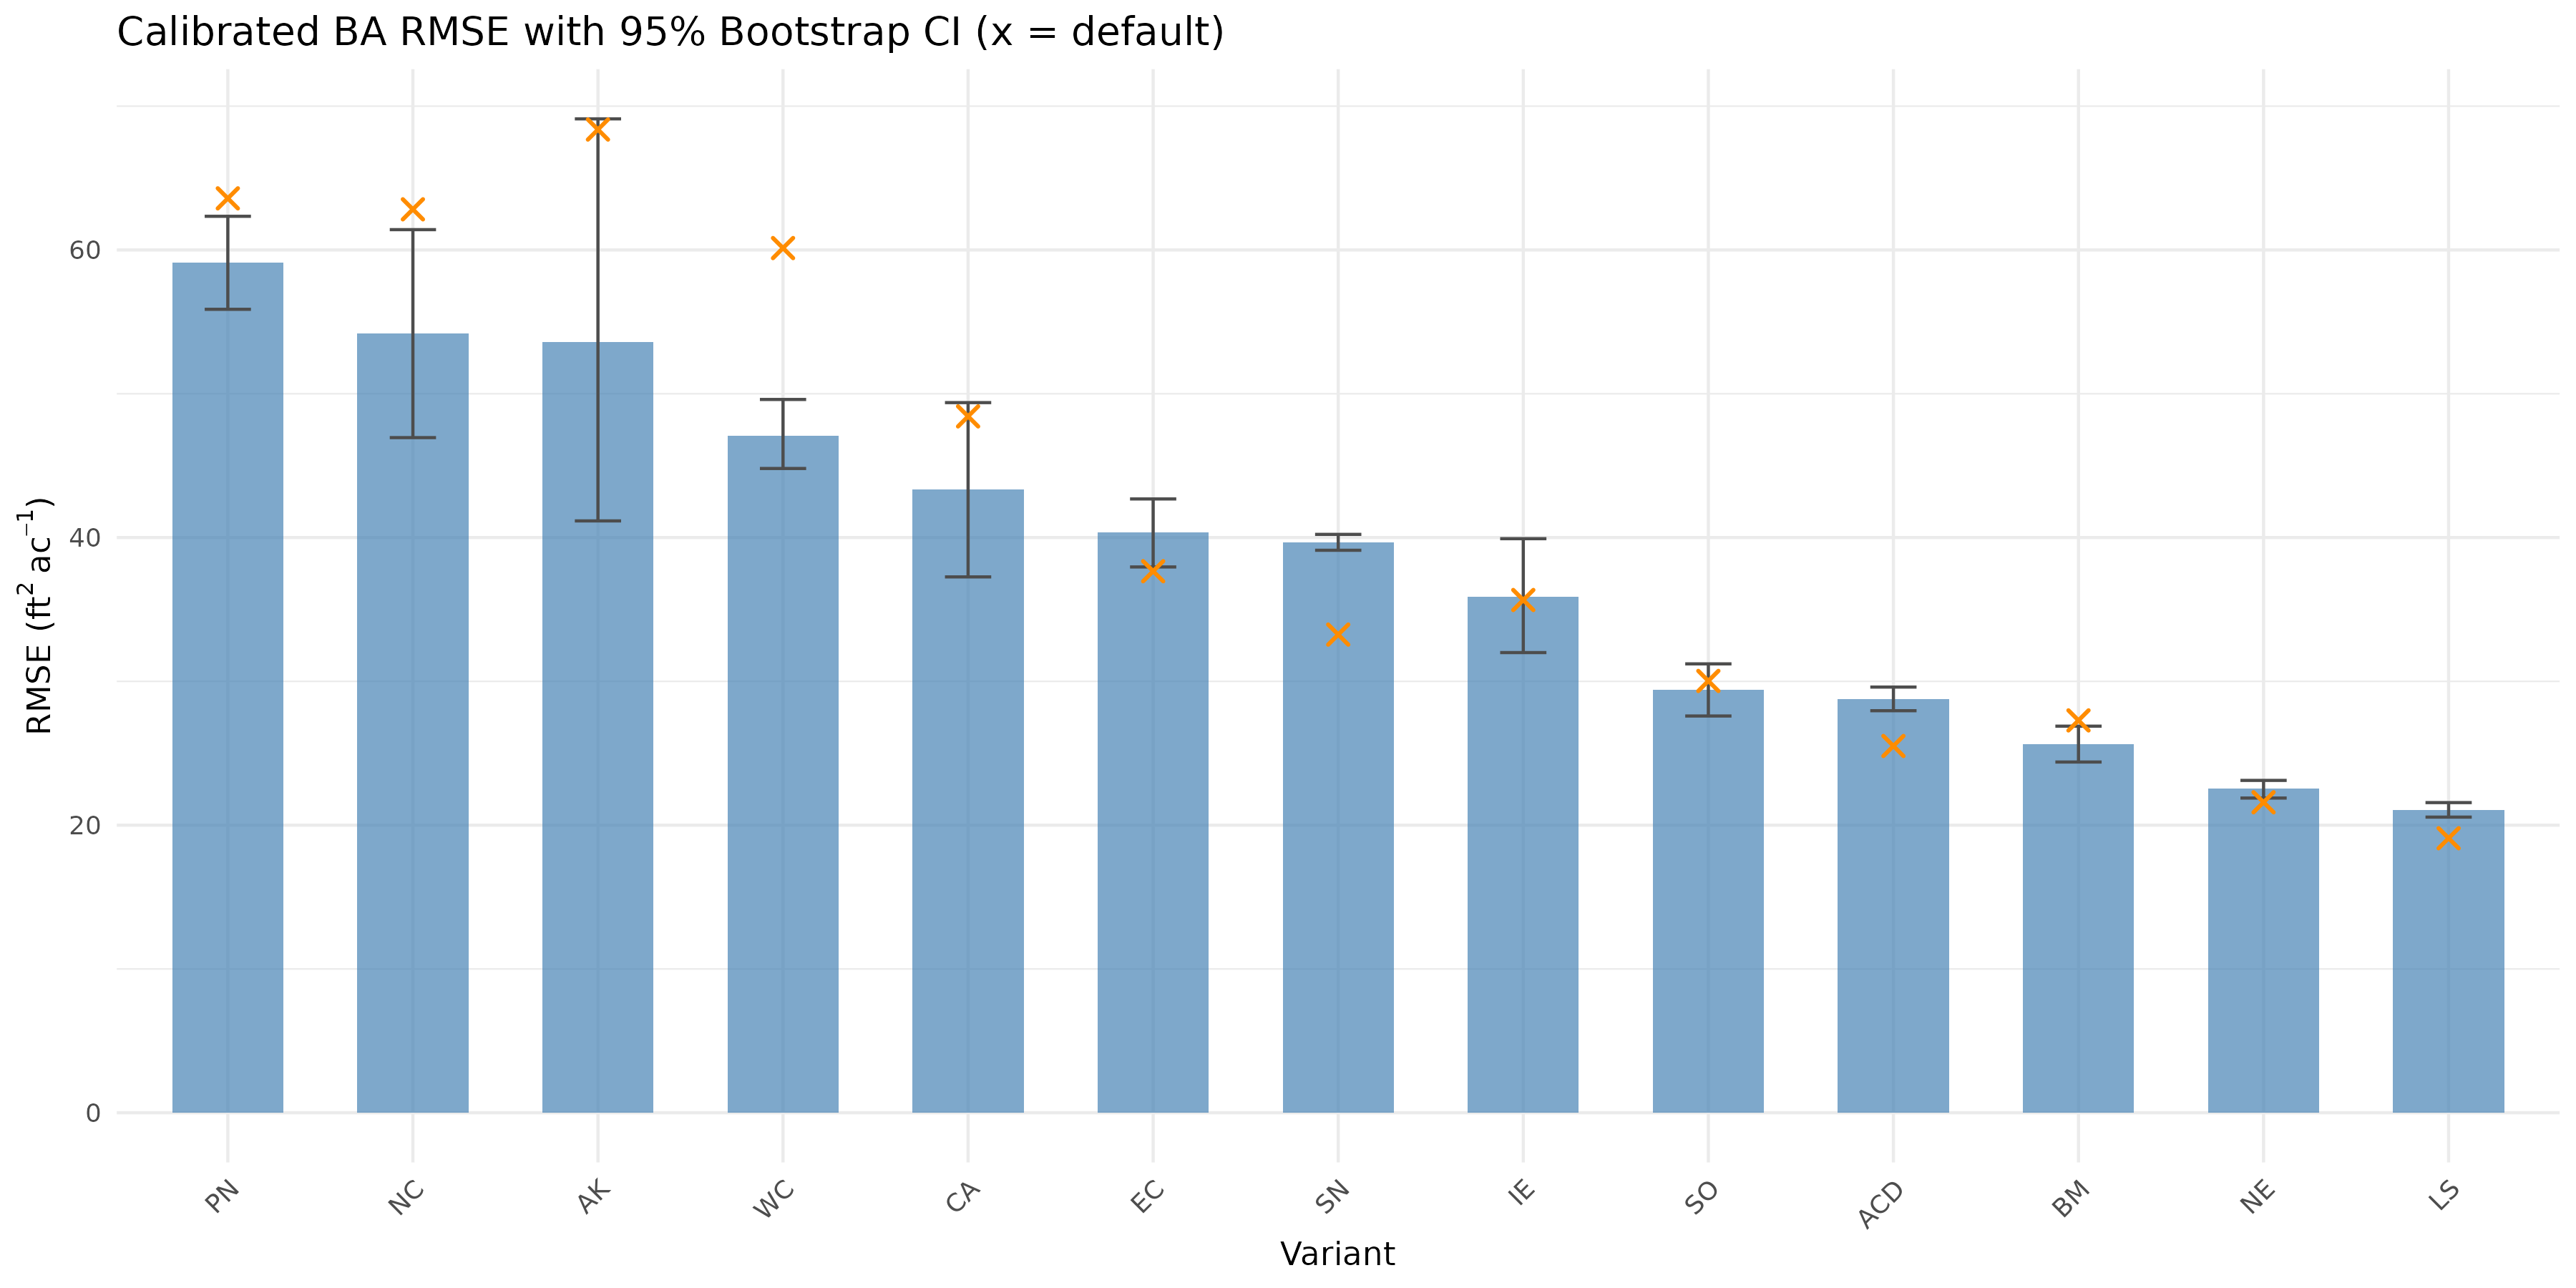
\includegraphics[width=0.90\textwidth]{14_ba_rmse_bootstrap_ci.png}
\end{center}

\vspace{0.2cm}
\begin{columns}[T]
\begin{column}{0.48\textwidth}
\begin{beamercolorbox}[rounded=true,shadow=true,wd=\textwidth]{block title}
\centering Calibrated RMSE: 15--60 ft$^2$/ac with narrow CIs
\end{beamercolorbox}
\end{column}
\begin{column}{0.48\textwidth}
\begin{beamercolorbox}[rounded=true,shadow=true,wd=\textwidth]{block title}
\centering Default ($\times$) often outside calibrated 95\% CI
\end{beamercolorbox}
\end{column}
\end{columns}
\end{frame}

% ============================================================================
% SLIDE 6: Projection Uncertainty
% ============================================================================
\begin{frame}
\frametitle{50--Year Projections: Uncertainty Quantification}

\vspace{-0.3cm}
\begin{center}
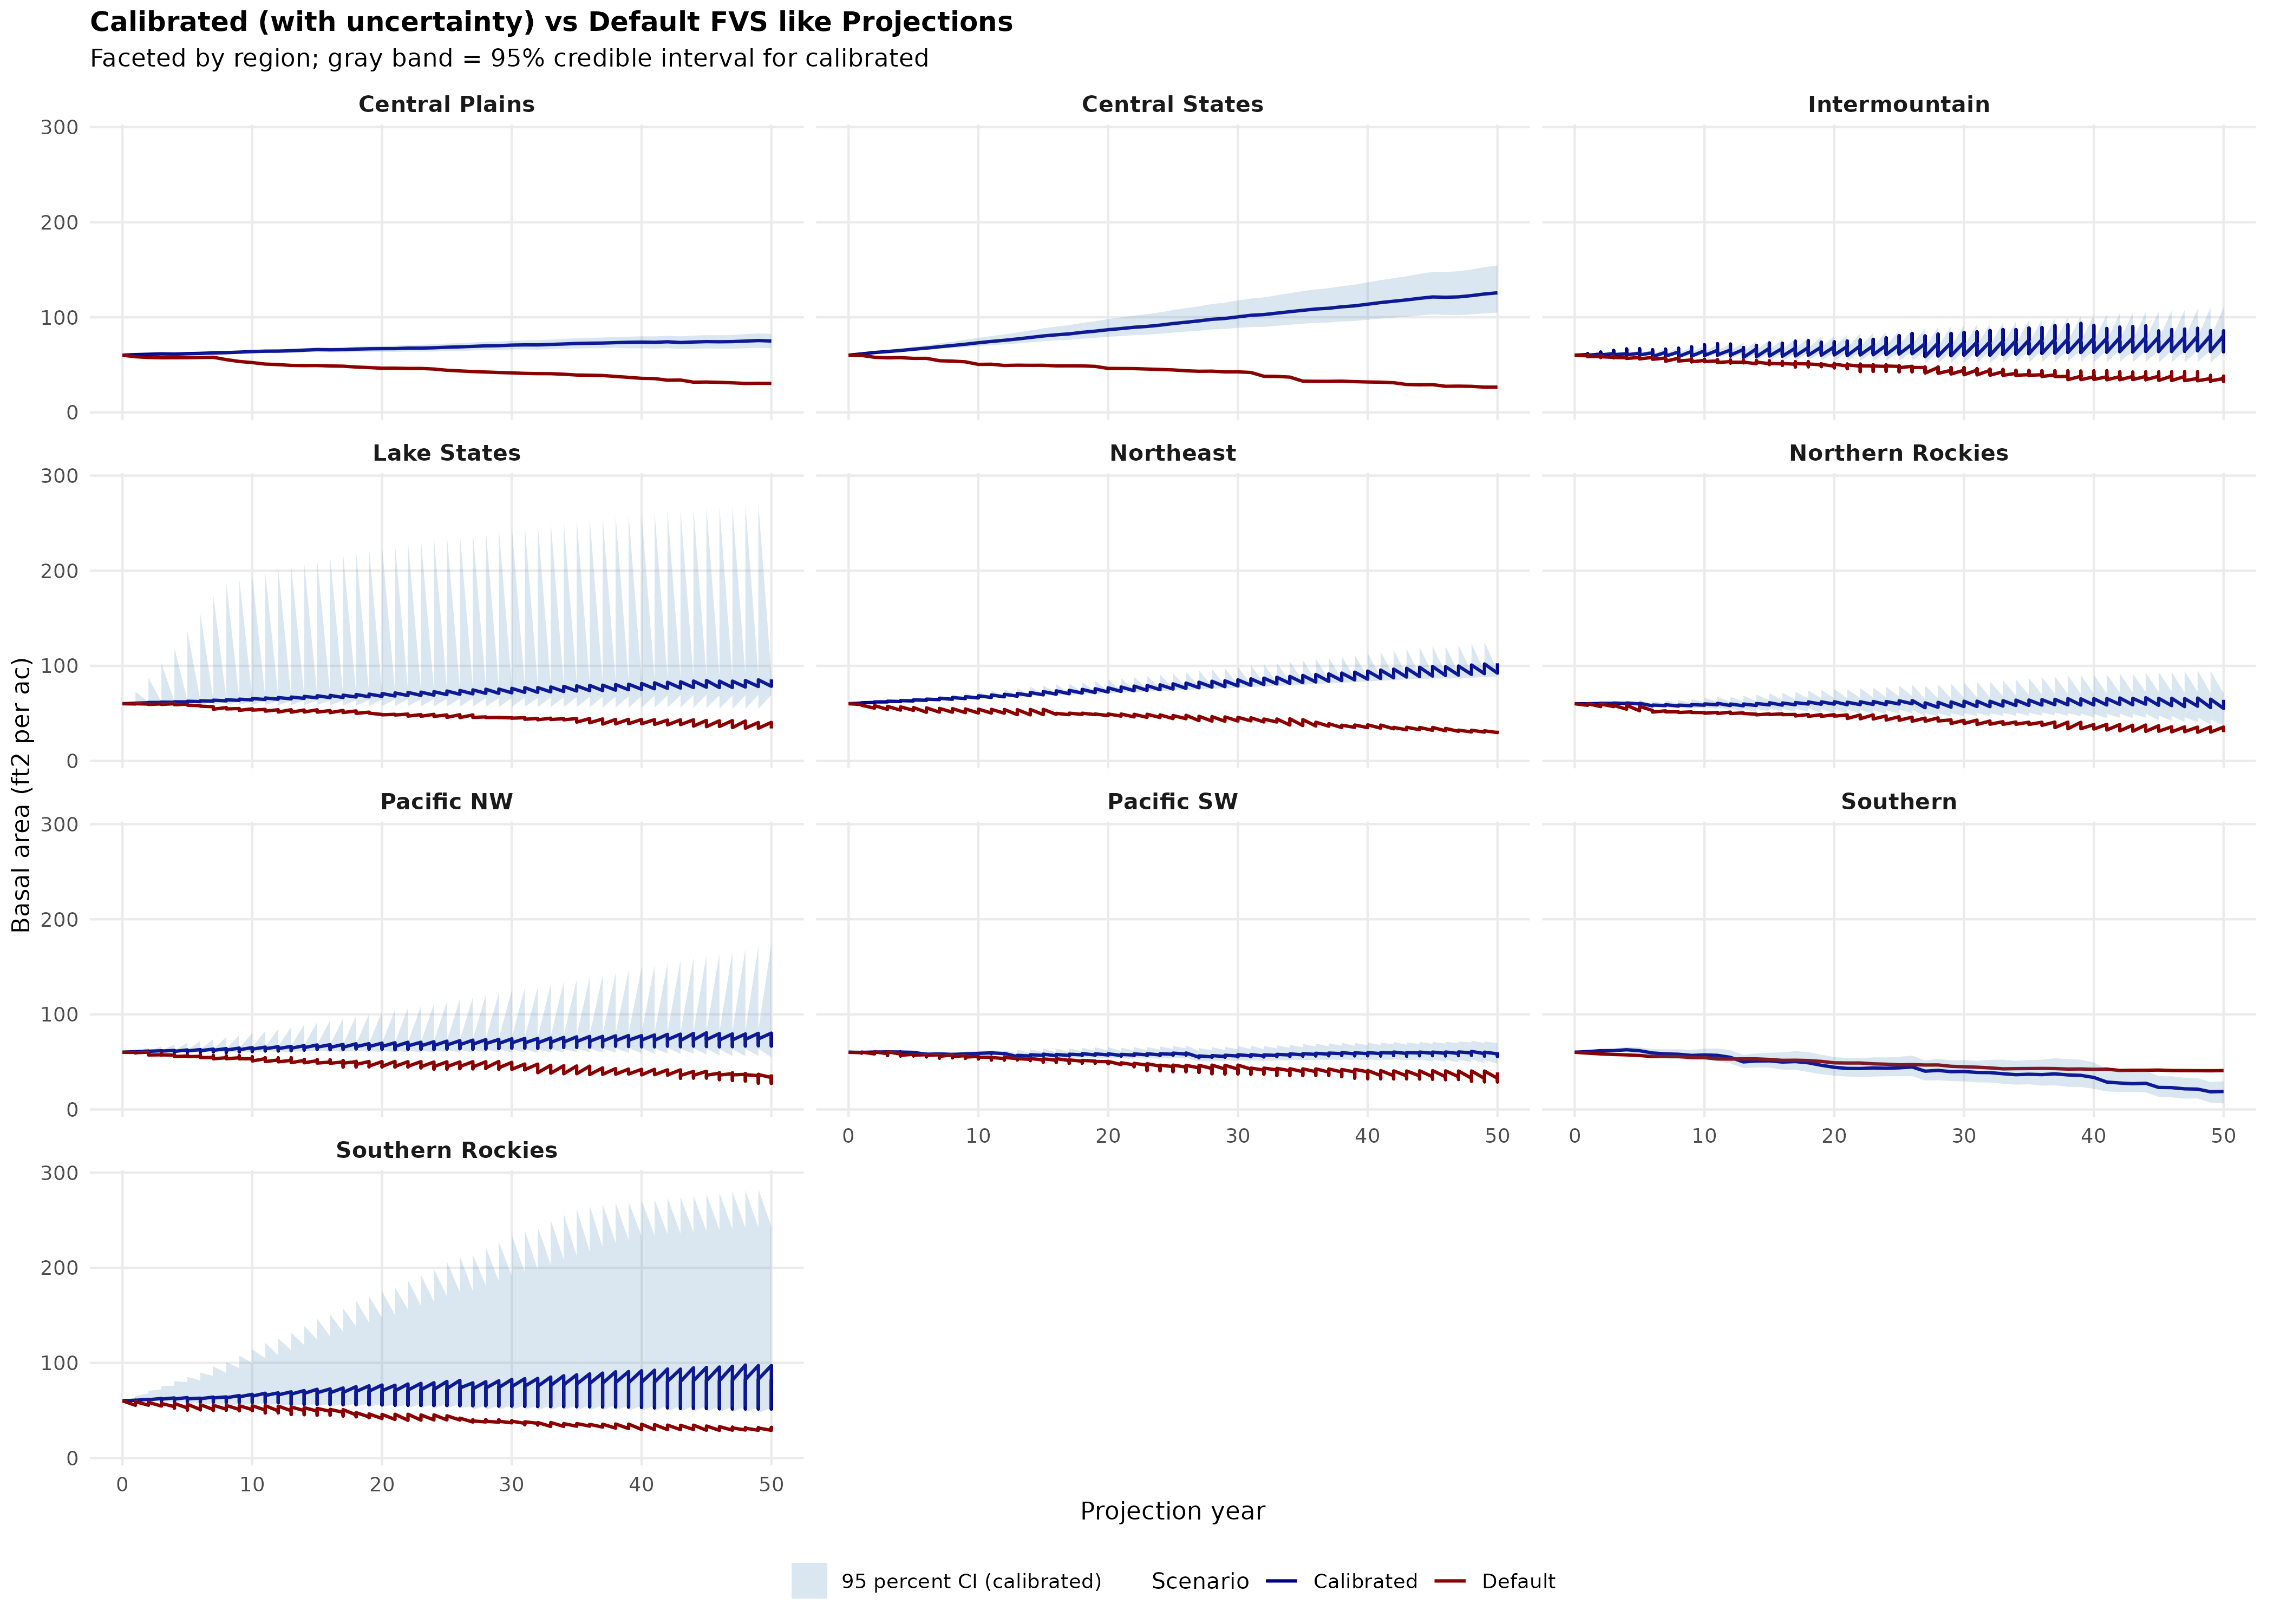
\includegraphics[width=0.88\textwidth,height=0.72\textheight,keepaspectratio]{fig_calibrated_vs_default_with_ci.png}
\end{center}

\vspace{-0.2cm}
{\scriptsize\color{fvsmuted} Blue bands = 95\% credible interval from Bayesian posteriors. Default FVS (red) frequently falls outside the calibrated CI, particularly in western variants.}
\end{frame}

% ============================================================================
% SLIDE 7: Remaining Gaps and Path Forward
% ============================================================================
\begin{frame}
\frametitle{Remaining Gaps and the Path Forward}

\begin{columns}[T]
\begin{column}{0.48\textwidth}
\begin{block}{\centering What Needs Work}
\begin{itemize}
  \item PAI predictions poor without ingrowth model\\
    {\small\color{fvsgreen}\textit{$\rightarrow$ Now addressed with empirical FIA ingrowth}}
  \item SN variant remains weakest ($R^2 = 0.52$)
  \item Crown ratio modeling limited
  \item Site index inconsistencies across FIA
\end{itemize}
\end{block}
\end{column}

\begin{column}{0.48\textwidth}
\begin{block}{\centering Roadmap}
\begin{enumerate}
  \item Ingrowth model from FIA PREV\_TRE\_CN \checkmark
  \item Large--tree mortality via DBH quadratic \checkmark
  \item Alternative productivity variables (ClimateSI, RS)
  \item SN sub--region analysis
  \item Open collaboration via GitHub
\end{enumerate}
\end{block}
\end{column}
\end{columns}

\vspace{0.5cm}
\begin{center}
\colorbox{fvsdark}{\parbox{0.7\textwidth}{\centering\color{fvsmoss}\itshape\large A single growth module capable of projecting any species anywhere in CONUS.}}
\end{center}
\end{frame}

\end{document}
